\chapter{Cơ sở lý thuyết}
\section{Hệ điều hành Android và đặc điểm bảo mật}
Android là hệ điều hành mã nguồn mở được phát triển bởi Google, hiện chiếm thị phần lớn nhất trong lĩnh vực thiết bị di động. Android có kiến trúc dựa trên nhân Linux, hỗ trợ đa nhiệm, dễ dàng cài đặt ứng dụng từ Google Play hoặc nguồn bên ngoài (sideload).
Về mặt bảo mật, Android cung cấp một số cơ chế như:
LaTeX là một hệ thống soạn thảo văn bản khoa học mạnh mẽ, đặc biệt hữu ích cho viết báo cáo, luận văn, và bài báo nghiên cứu.

\begin{itemize}
    \item Sandboxing: mỗi ứng dụng chạy trong một môi trường biệt lập.
    \item Permission system: kiểm soát quyền truy cập vào tài nguyên (SMS, Camera, Contact...).
    \item Application signing: các ứng dụng cần có chữ ký số để đảm bảo tính xác thực.
\end{itemize}

Tuy nhiên, do tính mở và sự đa dạng thiết bị, hệ sinh thái Android tồn tại nhiều lỗ hổng, khiến người dùng dễ dàng trở thành mục tiêu tấn công.

\section{Mã độc Android: khái niệm và kỹ thuật tấn công phổ biến}

\textbf{Mã độc Android (Android Malware)}\cite{10.1145/3503463} là các ứng dụng có hành vi độc hại, được cài đặt lên thiết bị nhằm đánh cắp thông tin, chiếm quyền điều khiển hoặc gây thiệt hại cho người dùng.

Phân loại mã độc Android phổ biến:
\begin{itemize}
    \item Adware: hiển thị quảng cáo không mong muốn.
    \item Spyware: theo dõi, đánh cắp thông tin cá nhân, vị trí, tin nhắn.
    \item Ransomware: mã hóa dữ liệu và đòi tiền chuộc.
    \item Trojan: giả dạng ứng dụng hợp pháp để phát tán mã độc.
    \item Botnet malware: biến thiết bị thành nút trong mạng tấn công phân tán.
\end{itemize}

Một số kỹ thuật tấn công thường gặp:
\begin{itemize}
    \item Privilege escalation: khai thác lỗ hổng để tăng quyền truy cập.
    \item Obfuscation \& Packing: làm rối mã nguồn, đóng gói để né tránh phát hiện.
    \item Phishing overlay: giả mạo giao diện đăng nhập để đánh cắp thông tin.
\end{itemize}

\begin{verbatim}
\begin{figure}[h]
    \centering
    \includegraphics[width=0.7\linewidth]{example-image} % tên file ảnh, không cần đuôi
    \caption{Ví dụ chèn hình ảnh trong LaTeX}
    \label{fig:example}
\end{figure}
Mã độc Android (Android Malware) là các ứng dụng có hành vi độc hại, được cài đặt lên thiết bị nhằm đánh cắp thông tin, chiếm quyền điều khiển hoặc gây thiệt hại cho người dùng.

\end{verbatim}

\begin{figure}[h]
    \centering
    \includegraphics[width=0.7\linewidth]{example-image} % tên file ảnh, không cần đuôi
    \caption{Ví dụ chèn hình ảnh trong LaTeX}
    \label{fig:example}
\end{figure}

\begin{verbatim}
Như minh họa ở Hình~\ref{fig:example}.
\end{verbatim}

Như minh họa ở Hình~\ref{fig:example}.

\section{Chèn bảng}

\begin{verbatim}
\begin{table}[h]
    \centering
    \caption{Ví dụ bảng trong LaTeX}
    \begin{tabular}{l c r}
        \toprule
        Cột 1 & Cột 2 & Cột 3 \\
        \midrule
        Trái  & Giữa  & Phải  \\
        A     & B     & C     \\
        \bottomrule
    \end{tabular}
    \label{tab:example}
\end{table}
\end{verbatim}

\begin{table}[h]
    \centering
    \caption{Ví dụ bảng trong LaTeX}
    \begin{tabular}{l c r}
        \toprule
        Cột 1 & Cột 2 & Cột 3 \\
        \midrule
        Trái  & Giữa  & Phải  \\
        A     & B     & C     \\
        \bottomrule
    \end{tabular}
    \label{tab:example}
\end{table}


Hệ thống phát hiện xâm nhập (Intrusion Detection System $-$ IDS) được thực hiện bởi Denning (1987), và kể từ đó IDS trở thành một lĩnh vực nghiên cứu nóng, như là một công cụ trong an ninh mạng máy tính. Thiết bị IDS có thể là phần cứng, phần mềm, hoặc kết hợp cả hai để theo dõi mạng máy tính và chống lại các truy cập trái phép. Mục tiêu chính của IDS là phát hiện được các cuộc tấn công trước khi chúng gây ra bất kỳ thiệt hại nghiêm trọng nào cho hệ thống mạng máy tính.

\subsection{Định nghĩa}

Đối với IDS, xâm nhập có nghĩa là cố gắng truy cập thông tin về hệ thống máy tính hoặc làm hỏng hoạt động của hệ thống theo cách bất hợp pháp hoặc trái phép. IDS là một ứng dụng bảo mật máy tính nhằm phát hiện một loạt các vi phạm bảo mật, từ các vụ đột nhập do người ngoài cố gắng xâm nhập và lạm dụng hệ thống bởi người trong cuộc [5]. Các chức năng chính của IDS là giám sát máy chủ và mạng, phân tích hành vi của hệ thống máy tính, tạo cảnh báo và phản hồi các hành vi đáng ngờ. Vì chúng giám sát các máy chủ và mạng liên quan, IDS thường được triển khai gần các nút mạng được bảo vệ (ví dụ: các bộ chuyển mạch trong các phân đoạn mạng chính).
%~\cite{viet1} \cite{eng1}

\begin{verbatim}
\begin{figure}[H] % [H] = cố định vị trí hình (cần \usepackage{float})
    \centering
    % Chèn ảnh, chỉnh kích thước bằng width
    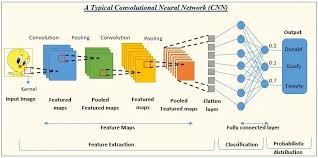
\includegraphics[width=\linewidth]{assets/cnn.jpeg}
    % Chú thích hình (tự động đánh số)
    \caption{Mô hình mạng CNN}
    % Nhãn để tham chiếu trong bài viết
    \label{fig:cnn-model}
\end{figure}
\end{verbatim}


\begin{figure}[htpb!]
    \centering
    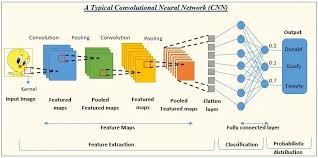
\includegraphics[width=1\linewidth]{assets/cnn.jpeg}
    \caption{Mô hình mạng CNN}
    \label{fig:enter-label}
\end{figure}

Có hai loại phương pháp phân loại IDS: phương pháp dựa trên chữ ký và phương pháp dựa trên nguồn dữ liệu. Trong số các phương pháp dựa trên phát hiện, IDS có thể được chia thành phát hiện lạm dụng và phát hiện bất thường. Trong số các phương thức dựa trên nguồn dữ liệu, IDS có thể được chia thành các phương thức dựa trên máy chủ và dựa trên mạng [6].

\subsection{Phân loại IDS dựa trên chữ ký}
Ý tưởng cơ bản để thể hiện các hành vi tấn công dựa trên chữ ký là quá trình phát hiện khớp với chữ ký của các mẫu bằng cơ sở dữ liệu chữ ký. Vấn đề chính trong việc xây dựng các hệ thống phát hiện dựa trên chữ ký là thiết kế chữ ký hiệu quả. Ưu điểm của phát hiện dựa trên chữ ký là nó có tỷ lệ cảnh báo giả thấp và báo cáo các loại tấn công cũng như các lý do một cách chi tiết. Nhược điểm của nó là có tỷ lệ báo động (missed alarm rate) bị bỏ lỡ cao, thiếu khả năng phát hiện các cuộc tấn công không xác định và yêu cầu duy trì một cơ sở dữ liệu chữ ký khổng lồ. 

Ý tưởng thiết kế đằng sau phát hiện bất thường là thiết lập một hồ sơ hành vi bình thường và sau đó xác định các hành vi bất thường bằng mức độ sai lệch của chúng so với hồ sơ bình thường. Do đó, chìa khóa để thiết kế một hệ thống phát hiện bất thường là xác định rõ ràng một cấu hình bình thường. Lợi ích của việc phát hiện bất thường là khả năng khái quát mạnh mẽ và khả năng nhận ra các cuộc tấn công chưa biết, trong khi thiếu sót của nó là tỷ lệ báo động sai cao và không thể đưa ra lý do có thể gây ra sự bất thường. Sự khác biệt chính giữa phát hiện dựa trên chữ ký và phát hiện bất thường được liệt kê trong Bảng 1.1. 

\begin{table}[ht]
  \centering
  \caption{Sự khác nhau giữa phát hiện dựa trên chữ ký và phát hiện bất thường [7]}
  \label{tab:signature-vs-anomaly}
  \renewcommand{\arraystretch}{1.15}
  \begin{tabularx}{\textwidth}{%
      >{\raggedright\arraybackslash}p{0.27\textwidth}
      >{\raggedright\arraybackslash}X
      >{\raggedright\arraybackslash}X}
    \toprule
    \textbf{Tiêu chí} &
    \textbf{Phát hiện dựa trên chữ ký} &
    \textbf{Phát hiện bất thường} \\
    \midrule
    Hiệu suất phát hiện &
    Tỷ lệ cảnh báo giả thấp; tỷ lệ báo động bỏ lỡ cao. &
    Tỷ lệ báo động bỏ lỡ thấp; tỷ lệ báo động sai cao. \\
    Hiệu quả phát hiện &
    Cao, nhưng giảm theo quy mô của cơ sở dữ liệu chữ ký. &
    Phụ thuộc vào độ phức tạp của mô hình. \\
    Phụ thuộc vào miền tri thức &
    Hầu như tất cả các phát hiện phụ thuộc vào miền tri thức. &
    Chỉ dựa vào đặc trưng dữ liệu. \\
    Khả năng diễn giải &
    Thiết kế dựa trên miền tri thức, khả năng diễn giải mạnh. &
    Chủ yếu đưa ra kết quả phát hiện; khả năng diễn giải yếu. \\
    Phát hiện tấn công không xác định &
    Chỉ phát hiện các cuộc tấn công đã biết. &
    Có thể phát hiện cả các cuộc tấn công đã biết và chưa biết. \\
    \bottomrule
  \end{tabularx}
\end{table}

Trong phân loại dựa trên phương pháp phát hiện, phát hiện dựa trên chữ ký bao gồm phương pháp dựa trên mẫu phù hợp, hệ thống chuyên gia và phương pháp dựa trên máy trạng thái hữu hạn. Phát hiện bất thường bao gồm các phương pháp dựa trên mô hình thống kê, dựa trên học máy và dựa trên chuỗi thời gian.

\subsection{Phân loại IDS dựa trên nguồn dữ liệu}
Một lợi thế của IDS dựa trên máy chủ (Host-Based IDS – HIDS) là nó có thể xác định chính xác các cuộc xâm nhập và bắt đầu phản hồi vì các IDS đó có thể giám sát hành vi của các đối tượng quan trọng (ví dụ: các tệp, chương trình và các cổng nhạy cảm). Nhược điểm là HIDS là chiếm tài nguyên máy chủ, phụ thuộc vào độ tin cậy của máy chủ và không thể phát hiện các cuộc tấn công mạng. 

Như hình minh hoạ cho chương trình codetour là Hình~\ref{fig:hinhanhminhhoa1}
\begin{figure}
    \centering
    
\includegraphics[width=1\linewidth]{figures/social-thumbnail.png}
    \caption{Tên minh hoạ cho ảnh này}
    \label{fig:hinhanhminhhoa1}
\end{figure}

IDS dựa trên mạng (Network-Based IDS – NIDS) thường được triển khai trên các máy chủ hoặc thiết bị chuyển mạch chính. Phần lớn các NIDS độc lập với hệ điều hành. Do đó, chúng có thể được áp dụng trong các hệ điều hành khác nhau. Hơn nữa, NIDS có thể phát hiện các loại tấn công mạng và giao thức cụ thể. Hạn chế là chúng chỉ giám sát lưu lượng đi qua một phân đoạn mạng cụ thể. Sự khác biệt chính giữa IDS dựa trên máy chủ và IDS dựa trên mạng được liệt kê trong Bảng \ref{tab:hids-vs-nids}.

\begin{table}[htpb!]
  \centering
  \caption{So sánh Host-Based IDS và Network-Based IDS}
  \label{tab:hids-vs-nids}
  \renewcommand{\arraystretch}{1.15}
  \begin{tabularx}{\textwidth}{%
      >{\raggedright\arraybackslash}p{0.27\textwidth}
      >{\raggedright\arraybackslash}X
      >{\raggedright\arraybackslash}X}
    \toprule
    \textbf{Tiêu chí} & \textbf{Host-Based IDS (HIDS)} & \textbf{Network-Based IDS (NIDS)} \\
    \midrule
    Nguồn dữ liệu &
    Nhật ký hệ điều hành hoặc chương trình ứng dụng. &
    Lưu lượng truy cập mạng. \\
    Triển khai &
    Cài trên từng máy chủ; phụ thuộc hệ điều hành; khó triển khai. &
    Đặt tại các nút mạng chính; triển khai tương đối dễ. \\
    Hiệu quả phát hiện &
    Thấp do phải xử lý nhiều nhật ký. &
    Cao, có thể phát hiện tấn công theo thời gian thực. \\
    Truy xuất nguồn gốc &
    Theo dõi quá trình xâm nhập theo đường dẫn gọi hệ thống. &
    Theo dõi vị trí và thời gian xâm nhập theo địa chỉ IP và dấu thời gian. \\
    Giới hạn &
    Không thể phân tích hành vi mạng. &
    Chỉ giám sát lưu lượng đi qua một phân đoạn mạng cụ thể. \\
    \bottomrule
  \end{tabularx}
\end{table}

\section{Tổng quan về học sâu}
Có hai loại học máy chính: học có giám sát và học không giám sát. Học có giám sát dựa vào thông tin hữu ích trong bộ dữ liệu được gắn nhãn. Phân loại là nhiệm vụ phổ biến nhất trong học có giám sát (và cũng được sử dụng thường xuyên nhất trong IDS). Tuy nhiên, việc ghi nhãn dữ liệu theo cách thủ công rất tốn kém và mất thời gian. Do đó, việc thiếu dữ liệu được dán nhãn đầy đủ tạo thành nút thắt chính cho việc học có giám sát. Ngược lại, học không có giám sát trích xuất thông tin đặc trưng có giá trị từ dữ liệu không được gắn nhãn, giúp việc lấy dữ liệu huấn luyện dễ dàng hơn nhiều. Tuy nhiên, hiệu suất phát hiện của các phương pháp huấn luyện không giám sát thường kém hơn so với các phương pháp huấn luyện có giám sát. Các thuật toán học máy phổ biến được sử dụng trong IDS được thể hiện trong Hình 1.1.

Học sâu (Deep Learing - DL) được phát triển từ mạng nơ-ron nhân tạo và hiện nay nó được chú trọng trong lĩnh vực học máy. Việc nghiên cứu mạng nơ-ron nhân tạo bắt đầu từ năm 1940. McCulloch và đồng sự, đề xuất mô hình McCulloch-Pitts bằng cách phân tích và tóm tắt nguyên lý của nơ-ron.

Deep Learning cho phép các mô hình tính toán bao gồm nhiều lớp xử lý để học biểu diễn dữ liệu với nhiều mức trừu tượng. Phương pháp này đã cải thiện đáng kể công nghệ tiên tiến trong nhận dạng giọng nói, nhận dạng đối tượng trực quan, phát hiện đối tượng và nhiều lĩnh vực khác như khám phá thuốc và bộ gen. Học sâu phát hiện ra cấu trúc phức tạp trong các tập dữ liệu lớn bằng cách sử dụng thuật toán back-propagation (lan truyền ngược) để chỉ ra cách một máy thay đổi các tham số bên trong để tính toán biểu diễn trong mỗi lớp. Deep learning đã mang lại những đột phá trong các ứng dụng xử lý hình ảnh, video, nhận dạng giọng nói và âm thanh [8]. 

\subsection{Định nghĩa về mạng nơ-ron}
Mạng nơ-ron là tập hợp các thuật toán, mô hình hóa như bộ não con người, được thiết kế để nhận diện mẫu. Nó diễn tả dữ liệu thông qua một loạt nhận thức máy tính, dán nhãn, hoặc phân nhóm đầu vào. Các mẫu mà nó nhận diện là dạng số, thể hiện dưới dạng các véc-tơ, tất cả là dữ liệu trong thế giới thực, có thể là hình ảnh, âm thanh, văn bản.

Mạng nơ$-$ron giúp chúng ta phân cụm, phân loại. Có thể nghĩ nó như là một lớp phân cụm, phân loại trên phía đầu của dữ liệu mà chúng ta lưu trữ và quản lý. Nó giúp gom nhóm các dữ liệu chưa có dán nhãn theo độ tương tự giữa các đầu vào, và nó phân loại dữ liệu khi có một tập dữ liệu được gán nhãn để huấn luyện.

\subsection{Các thành phần của mang nơ-ron cơ bản}
Mạng lưới nơ-ron được thiết kế đặc biệt dựa trên hoạt động bên trong của bộ não sinh học. Những mô hình này bắt chước các chức năng của các nơ-ron liên kết với nhau bằng cách chuyển các đặc trưng đầu vào thông qua một số lớp được gọi là perceptron (nơ-ron thần kinh), mỗi biến đổi đầu vào sử dụng một tập hợp các hàm. Phần này sẽ giải thích các thành phần của một perceptron, thành phần nhỏ nhất của mạng lưới thần kinh.

Một perceptron (nơ-ron thần kinh) thường được tạo thành từ ba phép toán chính: phép nhân vô hướng, phép tính tổng, và sau đó là một phép biến đổi sử dụng một phương trình riêng biệt gọi là hàm kích hoạt. Vì một perceptron đại diện cho một nơ$-$ron duy nhất trong não, chúng ta có thể kết hợp nhiều perceptron để đại diện cho một bộ não. Nó được gọi là một mạng nơ-ron.

\subsubsection{Đầu vào}
Các đầu vào chỉ đơn giản là các đặc trưng của chúng. Ví dụ, đối với một mẫu dữ liệu mạng, đây sẽ là một mảng các giá trị cho mỗi phép đo. Chúng có thể có đầu vào là: [24.2956, 8.375, 30.177547, 11.830604] đại diện cho thời gian gói tin từ nguồn đi, thời gian gói tin ở đích, jitter ở nguồn, jitter ở đích. Những đầu vào này là những gì sẽ được sửa đổi bởi perceptron.

\subsubsection{Trọng số}
Trọng số đại diện cho phép nhân vô hướng. Công việc của nó là đánh giá tầm quan trọng của từng đầu vào, cũng như tính định hướng. Theo ví dụ trên, jitter nguồn đóng góp nhiều hay ít cho việc phát hiện bất thường? Tìm ra các trọng số này là một nhiệm vụ rất khó khăn, và có nhiều giá trị khác nhau để thử.

\subsection{Hàm truyền}
Hàm truyền khác với các thành phần khác ở chỗ nó cần nhiều đầu vào. Công việc của hàm truyền là kết hợp nhiều đầu vào thành một giá trị đầu ra và đầu ra này được đưa vào hàm kích hoạt.

\subsubsection{Bias}
Đây là một đầu vào bổ sung. Đầu vào này luôn giữ nguyên trong mỗi perceptron. Nó được nhân với trọng số giống như các đầu vào khác, và mục đích của nó là cho phép giá trị trước khi hàm kích hoạt được chuyển lên và xuống, độc lập với chính các đầu vào. Điều này cho phép các trọng số khác cụ thể hơn vì chúng không phải cố gắng cân bằng tổng xung quanh giá trị 0.

\subsubsection{Hàm kích hoạt}
Hàm kích hoạt sẽ chuyển đổi số từ hàm truyền thành giá trị cho đầu vào tiếp theo. Thông thường, hàm kích hoạt là hàm phi tuyến. 